\part{Programming languages and paradigms}
\frame{\partpage}

\begin{frame}{What is a programming language?}
	\begin{itemize}
		\pause\item A \textbf{program} is a sequence of instructions for a computer to perform a specific task
		\pause\item A \textbf{programming language} is a formal language for communicating these sequences of instructions
	\end{itemize}
\end{frame}

\begin{frame}{Which is the best programming language?}
	\begin{itemize}
		\pause\item There is no ``best'' programming language
		\pause\item There are hundreds of programming languages, each better suited to some tasks than others
		\pause\item Sometimes your choice is dictated by your choice of platform, framework, game engine etc.
		\pause\item To become a better programmer (and maximise your employability)
			you should learn several languages (but one at a time!)
	\end{itemize}
\end{frame}

\begin{frame}{Low vs high level}
	\begin{itemize}
		\pause\item \textbf{Low level languages} give the programmer direct control over
			the hardware
		\pause\item \textbf{High level languages} give the programmer \textbf{abstraction},
			hiding the details of the hardware
		\pause\item High level languages trade efficiency for ease of programming
		\pause\item Lower level languages were once the choice of game programmers,
			but advances in hardware mean that higher level languages are often a
			better choice
	\end{itemize}
\end{frame}

\begin{frame}{Programming paradigms}
	\begin{itemize}
		\pause\item \textbf{Imperative}: program is a simple sequence of instructions,
			with \textbf{goto} instructions for program flow
		\pause\item \textbf{Structured}: like imperative, but with \textbf{control structures}
			(loops, conditionals etc.)
		\pause\item \textbf{Procedural}: structured program is broken down into
			\textbf{procedures}
		\pause\item \textbf{Object-oriented}: related procedures and data are grouped into
			\textbf{objects}
		\pause\item \textbf{Functional}: procedures are treated as mathematical objects that
			can be passed around and manipulated
		\pause\item \textbf{Declarative}: does not define the control flow of a program,
			but rather defines logical relations
	\end{itemize}
\end{frame}

\begin{frame}{Which paradigm?}
	\begin{itemize}
		\pause\item \textbf{Imperative} and \textbf{structured} languages are mainly of
			historical interest
		\pause\item Most commonly used languages today are a mixture of \textbf{procedural}
			and \textbf{object-oriented} paradigms, with many also incorporating
			ideas from \textbf{functional} programming
		\pause\item Purely \textbf{functional} languages are mainly used in academia,
			but favoured by some programmers
		\pause\item Purely \textbf{declarative} languages have uses in academia and some special-purpose languages
	\end{itemize}
\end{frame}

\begin{frame}{Machine code}
	\begin{columns}
		\begin{column}{0.4\textwidth}
			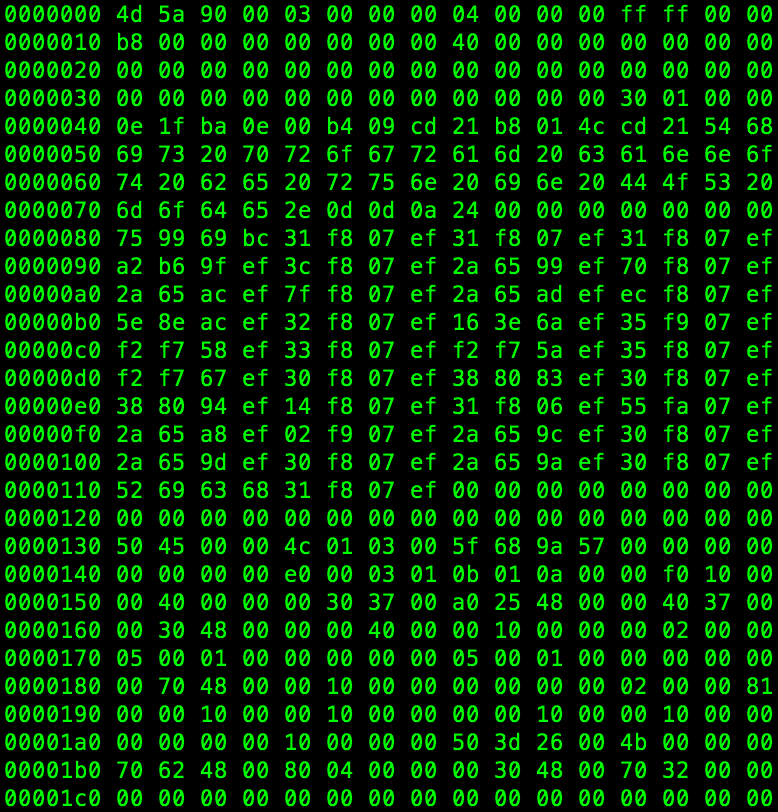
\includegraphics[width=\textwidth]{machinecode}
		\end{column}
		\begin{column}{0.58\textwidth}
			\begin{itemize}
				\pause\item Programs are represented as sequences of \textbf{numbers}
					specifying \textbf{machine instructions}
				\pause\item More on this later in the module
				\pause\item Nobody has actually written programs in machine code since the 1960s...
			\end{itemize}
		\end{column}
	\end{columns}
\end{frame}

\begin{frame}{Assembly language}
	\begin{columns}
		\begin{column}{0.4\textwidth}
			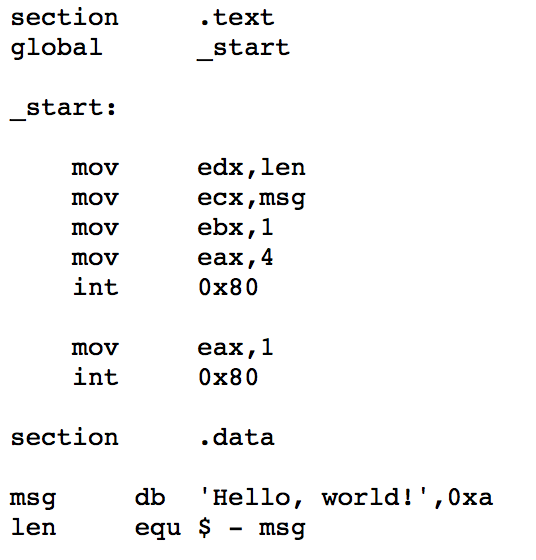
\includegraphics[width=\textwidth]{assembly}
		\end{column}
		\begin{column}{0.58\textwidth}
			\begin{itemize}
				\pause\item Each line of assembly code translates \textbf{directly} to an instruction of machine code
				\pause\item Commonly used for games in the 70s/80s/90s, but hardly ever used now
				\pause\item Allows very fine control over the hardware...
				\pause\item ... but difficult to use as there is no \textbf{abstraction}
				\pause\item Also not portable between CPU architectures
			\end{itemize}
		\end{column}
	\end{columns}
\end{frame}

\begin{frame}{C++}
	\begin{columns}
		\begin{column}{0.4\textwidth}
			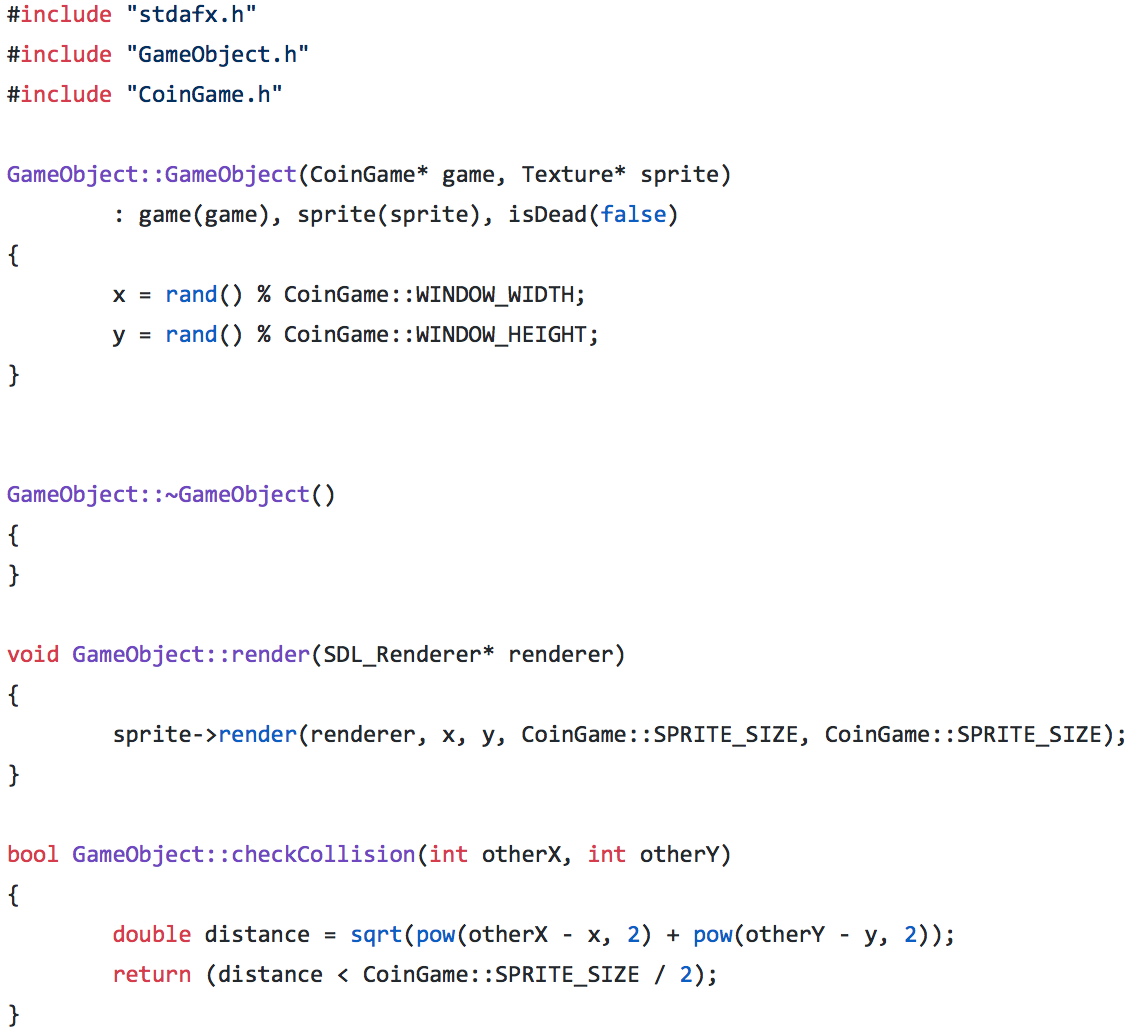
\includegraphics[width=\textwidth]{cplusplus}
		\end{column}
		\begin{column}{0.58\textwidth}
			\begin{itemize}
				\pause\item Initially an object-oriented extension for the procedural language C
				\pause\item Low level (though higher level than assembly)
				\pause\item Used by developers of game engines,
					and games using many popular ``AAA'' engines (Unreal, Source, CryEngine, ...)
				\pause\item Also used by developers of operating systems and embedded systems,
					but falling out of favour with other software developers
			\end{itemize}
		\end{column}
	\end{columns}
\end{frame}

\begin{frame}{High level languages}
	\pause Often favoured by smaller indie teams for rapid development
	\begin{itemize}
		\pause\item C\# (XNA, Unity)
		\pause\item Python (EVE Online, Pygame, Ren'py)
		\pause\item JavaScript (HTML5 browser games)
		\pause\item ActionScript (Flash games)
		\pause\item Objective-C, Swift (iOS games)
		\pause\item Java (Minecraft, Android games)
	\end{itemize}
	\pause There are many others, but these are the most commonly used in game development
\end{frame}

\begin{frame}{Scripting languages}
	\pause Many games use scripting languages in addition to their main development language
	\begin{itemize}
		\pause\item Lua (many AAA games)
		\pause\item Bespoke languages (many AAA games)
	\end{itemize}
	\pause Some game engines have their own scripting language
	\begin{itemize}
		\pause\item UnrealScript, Blueprint (Unreal Engine)
		\pause\item GML (GameMaker)
	\end{itemize}
\end{frame}

\begin{frame}{Visual programming languages}
	\begin{columns}
		\begin{column}{0.4\textwidth}
			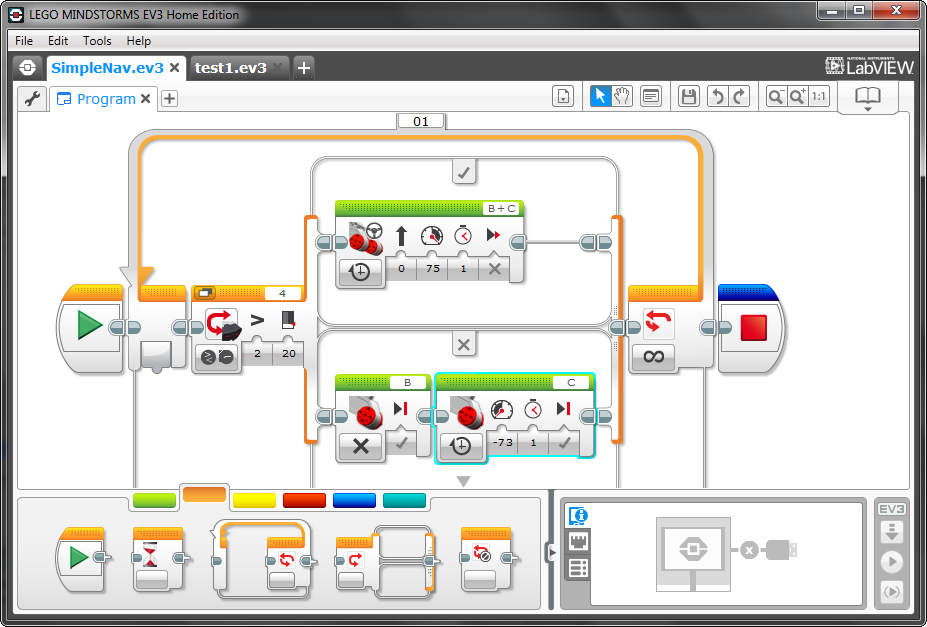
\includegraphics[width=\textwidth]{mindstorms}
			\par\vspace{2ex}\par
			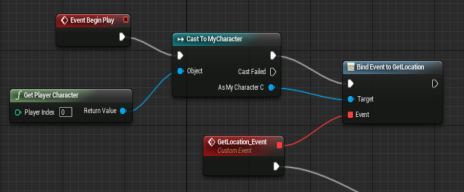
\includegraphics[width=\textwidth]{blueprint}
		\end{column}
		\begin{column}{0.58\textwidth}
			\pause Based on connecting graphical blocks rather than writing code as text
			\begin{itemize}
				\pause\item Scratch (used for teaching in school)
				\pause\item Lego Mindstorms
				\pause\item Blueprint (Unreal)
			\end{itemize}
			\pause Note: despite the name, Microsoft Visual Studio is \textbf{not}
				a visual programming environment!
		\end{column}
	\end{columns}
\end{frame}

\begin{frame}{Special purpose languages}
	\begin{itemize}
		\pause\item SQL (database queries)
		\pause\item GLSL, HLSL (GPU shader programs)
		\pause\item LEX, YACC (script interpreters)
	\end{itemize}
\end{frame}

\begin{frame}{Markup languages}
	\pause Not to be confused with programming languages...
	\begin{itemize}
		\pause\item HTML, CSS (web pages)
		\pause\item LaTeX, Markdown (documentation)
		\pause\item XML, JSON (data storage)
	\end{itemize}
\end{frame}

\begin{frame}{Which programming language is most popular?}
	\begin{center}
		\url{http://githut.info}
	\end{center}
\end{frame}

\begin{frame}{``Family tree'' of programming languages}
	\begin{center}
		\url{https://www.levenez.com/lang/lang.pdf}
	\end{center}
\end{frame}
